\begin{table*}
  \centering
  \caption{Target text-based Captcha schemes used in our experiment}
  \label{tab: captcha_show}
  \small
  \begin{tabular}{|c|c|c|c|c|c|}
    \hline
     &  &  & \multicolumn{2}{|c|}{Security Features} & \\
     \cline{4-5}
    \multirow{-2}{*}{Scheme} & \multirow{-2}{*}{Website} & \multirow{-2}{*}{Sample} & Anti-segmentation Features & Anti-recognition Features & \multirow{-2}{*}{Missing characters} \\
    \hline
    Google & google.com & \tabincell{c}{
\includegraphics[width=0.1\textwidth]{fig/experiment_captchas/google1.jpg}} & \tabincell{c}{ Overlapping characters, \\ only Enligh letters used} & \tabincell{c}{Varied font size, color, \\ rotating, disortion and waving used} & -- \\
    \hline
    Baidu & baidu.com & \tabincell{c}{
\includegraphics[width=0.1\textwidth]{fig/experiment_captchas/baidu3.jpg}} & \tabincell{c}{Connecting Lines, overlapping, \\ only Enligh letters used} & \tabincell{c}{Both hollow and solid characters, \\ varied font size, color, \\ rotating, disortion and waving used} & Z \\
    \hline
    Alipay & alipay.com & \tabincell{c}{
\includegraphics[width=0.1\textwidth]{fig/experiment_captchas/alipay1.jpg}} & \tabincell{c}{Overlapping characters used} & \tabincell{c}{Both English letters and \\ Arabic numerals, \\ rotating and distortion used} & 0, 1, I, L, O  \\
    \hline
     Wikipedia& wikipedia.org & \tabincell{c}{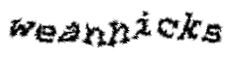
\includegraphics[width=0.1\textwidth]{fig/experiment_captchas/wikipedia1.png}} & \tabincell{c}{Only English letters used} & \tabincell{c}{Character rotating, \\ distortion and waving} & --  \\
     \hline
     Sohu& sohu.org & \tabincell{c}{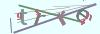
\includegraphics[width=0.1\textwidth]{fig/experiment_captchas/sohu1.jpg}} & \tabincell{c}{Complex background, \\ connection lines, \\and overlapping used} & \tabincell{c}{varied font size, color \\ and character rotating} & 0, 1, i, l, o, z  \\
    \hline
    %NetEase & 163.com & \tabincell{c}{
\includegraphics[width=0.1\textwidth]{fig/experiment_captchas/netease1.jpg} 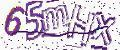
\includegraphics[width=0.1\textwidth]{fig/experiment_captchas/netease2.jpg}} & \tabincell{c}{Complex background, \\ connecting lines} & \tabincell{c}{Both hallow and solid characters, \\ varied rotating angles used} \\
%    \hline
%    VIPSHOP & vip.com & \tabincell{c}{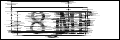
\includegraphics[width=0.1\textwidth]{fig/experiment_captchas/vipshop1.jpg} 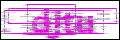
\includegraphics[width=0.1\textwidth]{fig/experiment_captchas/vipshop2.jpg}} & \tabincell{c}{Complex background, \\ overlapping characters} & \tabincell{c}{Both English letters \\ and Arabic numerals, \\ varied font colors used} \\
%    \hline
%     TOUP& tuniu.com & \tabincell{c}{ 
\includegraphics[width=0.1\textwidth]{fig/experiment_captchas/tuniu1.jpg} 
\includegraphics[width=0.1\textwidth]{fig/experiment_captchas/tuniu2.jpg}} & \tabincell{c}{Overlapping characters used} & \tabincell{c}{Both English letters \\ and Arabic numerals, \\ waving characters used} \\
%    \hline
  \end{tabular}
\end{table*}

\section{Experimental Setup}
\subsection{Data Preparation and Collection \label{section: captcha_collection}}
The captchas used in our evaluation are made up of both training data and testing data, and they come from two different sources. The training captchas are synthesized by our captcha synthesizer (Section~\ref{section: captcha_generator}) and the testing captchas are collected from target websites using a traditional mining method written through a python script.

\noindent \textbf{Target Websites.} We select the target websites based on the following rules: (1) the captchas of website combines at least one anti-segmentation and three anti-recognition features; (2) the website must have a large number of active users and (3) the target websites should cover as many industries as possible.
%(3) the testing Captchas are relatively easy to mine~\footnote{Some Captcha schemes, such as Tecent Captchas, are hard to mine as each Captcha image has a different URL.}.
According to the three factors, we target 18 famous websites for preparing our data. These target websites can be classified into 5 categories: \emph{E-commerce site} (such as Ebay, Alipay, JD and Alipayexpress), \emph{Social Networks} (such as Live and Sina Microblog), \emph{Search Engine} (such as Google, Baidu, 360 and Bing), \emph{Portal sites} (such as Wikipedia, Sohu and Sina) and other sites (such as Yutube and Microsoft Office).
 Table~\ref{tab: captcha_show} presents some captcha schemes of target websites and their security features.
 At last, we collected 11 captcha schemes because some websites share the same captcha scheme. For example, Yutube uses Google’s captcha, and Live, Office and Bing use Microsoft’s captcha. Through the analysis of these target captchas, we found that most schemes remove the similar characters such as o and 0, 1 and l, etc. The last column of Table~\ref{tab: captcha_show} presents the missing characters of some captcha schemes.
%\textcolor{red}{5 famous websites for preparing our data: Baidu, Alipay, NetEase, VIPSHOP and TOUP}.


\noindent \textbf{Synthesize Training Captchas.} 
To ensure the synthesized captcha as likely as the true one, we first manually label which security feature of the target captcha used as described in Section~\ref{section: captcha_generator}. According to the security features, our generator can synthesize adequate training captchas for training. In our experiment, we totally synthesized 11 kinds of captchas coming from the 18 famous websites (Section~\ref{section: captcha_collection}). For each type of captcha, we synthesized 20k for training the preprocessing model and synthesized 200k captchas for training the base model.

\noindent \textbf{Mine Testing Captchas.} 
The testing captchas used in our evaluation are automatically collected from the target websites using a python script. For each target website, we employ 500 real captchas for training the fine tune model and employ 200 for testing the efficiency of our attacking system. We recruited nine participants from our institution to manually mark the labels of the collected captchas. To decrease the marking error rate, the nine participants are divided into three groups and each group has three people. We choose these captchas which are correctly tagged by two participators at the same time as the testing captchas.

\subsection{Implementation}
Our preprocessing model is built upon a variant of \emph{Pix2Pix} framework~\cite{Pix2PixCode} in Tensorflow. The base model and fine tune model are built in Keras. The developed software ran on an ordinary server with a 3.2-GHz Inter Xeon CPU with 100-GB RAM and a TITAN Xp GPU. The operating system is Ubuntu 16.04.


%\subsection{Captchas Show}
